%!TEX root = ../thesis.tex
%*******************************************************************************
%*********************************** Fourth Chapter *****************************
%*******************************************************************************

\chapter{Architecture Search Literature Review}

\ifpdf
    \graphicspath{{Chapter4/Figs/Raster/}{Chapter4/Figs/PDF/}{Chapter4/Figs/}}
\else
    \graphicspath{{Chapter4/Figs/Vector/}{Chapter4/Figs/}}
\fi

The field of architecture search has received a significant burst of work in recent years. As the advances in computational power brought advances in the training of individual networks, the same power has lent itself to searching architectures of ever-larger networks. The need for automated methods has increased significantly as the size and complexity of model has increased. Simpler models with a small set of hyper-parameters that can be quickly varied and easily interpreted can be tuned by hand without significant investment of time. As models have grown to significant depths, e.g. \citet{DBLP:journals/corr/SzegedyIV16}, the task of tuning layer configuration, depth, and various other hyper-parameters has become somewhat of a "Dark Art", using mainly heuristic and architectures that have been show to be good on previous problems as a basis.

While there has been no direct application of these methods to Bayesian Neural Networks, the close analogy of Bayesian Neural Networks and their regular counterparts implies that much of the work of architecture search in regular neural networks could be applied to searching for architectures in Bayesian Neural Networks.

Since the work by \citet{zoph2016neural} there has been an explosion in the number of papers and methodologies that deal with this subject \citep{mendoza2016towards,Baker2016,zoph2016neural,miikkulainen2019evolving,Cai2018,Adam2019,Sciuto,Wang,Li,Bender2018,liu2018progressive,fusi2018probabilistic,zoph2018learning,liu2018darts,Pham2018,kandasamy2018neural,zhong2017practical,negrinho2017deeparchitect,cortes2017adanet,Brock2017,real2017large,liu2017hierarchical,xie2017genetic,jenatton2017bayesian,Zela2018}. Some work does exist before this, although a large portion of this work is limited to small scale neuro-evolution searches, the processes of starting with small networks and progressively growing them in a directed fashion through evolutionary algorithms, and early Bayesian Optimisation applications targeted at general machine learning hyper-parameter optimisation, rather than to specific architecture search \citep{swersky2014raiders,bergstra2013making,snoek2012practical,stanley2002evolving,kitano1990designing,zhang2016flash}.

The process of architecture search can be broken into three main steps: The Search Space, the Search Method, and the Evaluation Method. While in some methodologies the choice of one of these is necessitated by the choice of another, it is usually possible to separate the choices out. Figure \ref{fig:methods} summarises the various methodologies that have been utilised in recent work, and some of the choices that have to be made when designing a search method. Figure \ref{fig:AS_procedure} describes the abstract process of architecture search. The choices in search space are not mutually exclusive; larger architecture searches will generally constrain the search space in more than one way to reduce its size. The choice in Search Method and Evaluation Method are generally mutually exclusive.

Briefly, a review of these different sections to architecture search and the methodologies proposed.

\begin{figure}
	\centering
	{\def\arraystretch{2}
	\begin{tabular}{C{1.5in}cC{1.5in}cC{1.5in}}
		\textbf{Search Space} & \hspace{1cm} & \textbf{Search Method} & \hspace{1cm} & \textbf{Evaluation Method}\\
		\cline{1-1} \cline{3-3} \cline{5-5}
		Continuous vs Discrete & & Random search & &  Full training\\
		Unstructured vs Structured & & Evolutionary Strategies & & Partial Training \\
		Cell blocks & & Bayesian Optimisation & & One-shot models / Weight-sharing \\
		Meta-architectures & & Gradient based optimisation & & Weight inheritance / Network Morphism\\
		Restricted building block & & Reinforcement Learning & & Hyper-networks
	\end{tabular}
	}
	\caption{Various groupings of methodology choices explored by recent works in architecture search, broken into categories}
	\label{fig:methods}
\end{figure}

\begin{figure}
	\tikzstyle{block} = [rectangle, draw, 
	text width=6em, text centered, minimum height=5em]
	\centering
	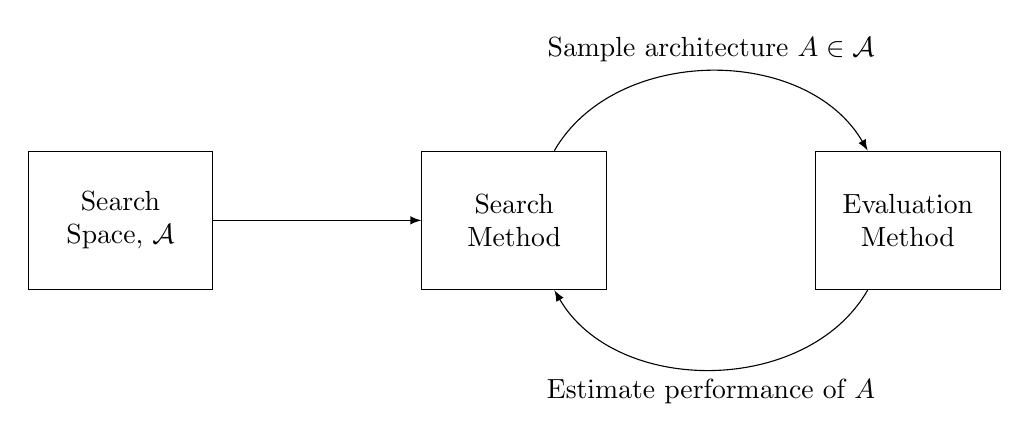
\begin{tikzpicture}[node distance = 5cm, auto]
	\node [block] (SS) {Search Space, \( \mathcal{A} \)};
	\node [block, right of=SS] (SM) {Search Method};
	\node [block, right of=SM] (EM) {Evaluation Method};
	
	\path[->]
	(SS) edge (SM);
	
	\path[->]
	(SM) edge [bend left=60] node [above] {Sample architecture \( A \in \mathcal{A} \)} (EM);
	
	\draw[->]
	(EM) edge [bend left=60] node [below] {Estimate performance of \( A \)} (SM);
	\end{tikzpicture}
	\caption{Abstract block diagram of the architecture search procedure. The search space defines a subset of all possible architectures \( \mathcal{A} \) to be searched over. The Search Method picks an architecture to sample from the search space to be evaluated by the Evaluation Method. The Evaluation Method returns the performance estimate to the Search Method.}
	\label{fig:AS_procedure}
\end{figure}

\section{Search Space}

The Search Space defines in principle the possible set of architectures that the search process might discover. The simplest of these are \textit{chain structure spaces}. These are simply a sequence of layers. The search space is characterised by the number of layers, the number of possible operations choosable at each layer, e.g. fully connected layers, convolutional layers etc., and the hyper-parameters associated with each layer e.g. number of filters, kernel size and strides for convolutions \citep{Baker2016,Cai2018,Suganuma}, or the number of units in fully connected layers \citep{mendoza2016towards}. Since the number of hyper-parameters are conditional on the choice of operation type, the search space descriptor will in general not be fixed length. Methods either deal with this conditional nature, or allow only certain choices of hyper-parameters for each layer type, fixing the descriptor length of the search space.

More recent works \cite{Brock2017,Elsken2018,zoph2018learning,Elsken2018a,Real,kandasamy2018neural} have introduced the ability to include more complex design elements such as skip connections to the search space which can build \textit{multi-branched structures}. The difference between this and simple feed forward structures is shown in figure \ref{fig:Search_spaces}. These search spaces are much more flexible, but are significantly larger.

\begin{figure}
	\tikzstyle{white} = [rectangle, draw, fill=White,
	text width=2em, text centered, minimum height=0.7em, font=\tiny]
	\tikzstyle{red} = [rectangle, draw, fill=Red!20!White,
	text width=2em, text centered, minimum height=0.7em, font=\tiny]
	\tikzstyle{blue} = [rectangle, draw, fill=Blue!20!White,
	text width=2em, text centered, minimum height=0.7em, font=\tiny]
	\tikzstyle{green} = [rectangle, draw, fill=Green!20!White,
	text width=2em, text centered, minimum height=0.7em, font=\tiny]
	\centering
	\begin{subfigure}{0.45\textwidth}
		\centering
		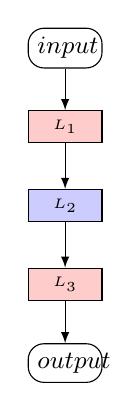
\begin{tikzpicture}[node distance = 1cm, auto]
		\node [white] (in) {\( input \)};
		\node [red, below of=in] (l1) {\( L_1 \)};
		\node [blue, below of=l1] (l2) {\( L_2 \)};
		\node [red, below of=l2] (l3) {\( L_3 \)};
		\node [white, below of=l3] (out) {\( output \)};
		
		\draw[->]
		(in) -- (l1);
		\draw[->]
		(l1) -- (l2);
		\draw[->]
		(l2) -> (l3);
		\draw[->]
		(l3) -> (out);
		
		\end{tikzpicture}	
		\caption{Chain structure search space}
	\end{subfigure}
	\begin{subfigure}{0.45\textwidth}
		\centering
		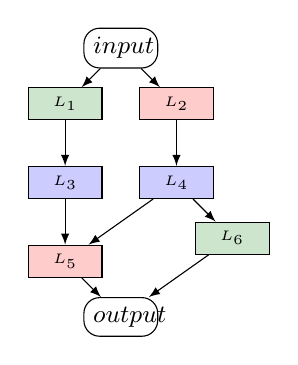
\begin{tikzpicture}[node distance = 1cm, auto]
		\node [white] (in) {\( input \)};
		\node [red, below right of=in] (l1) {\( L_2 \)};
		\node [green, below left of=in] (l11) {\( L_1 \)};
		\node [blue, below of=l1] (l2) {\( L_4 \)};
		\node [blue, below of=l11] (l22) {\( L_3 \)};
		\node [green, below right of=l2] (l3) {\( L_6 \)};
		\node [red, below of=l22] (l33) {\( L_5 \)};
		\node [white, below right of=l33] (out) {\( output \)};
		
		\draw[->]
		(in) -- (l1);
		\draw[->]
		(l1) -- (l2);
		\draw[->]
		(l2) -> (l3);
		\draw[->]
		(l3) -> (out);
		
		\draw[->]
		(in) -- (l11);
		\draw[->]
		(l11) -- (l22);
		\draw[->]
		(l22) -> (l33);
		\draw[->]
		(l33) -> (out);
		\draw[->]
		(l2) -> (l33);
		
		\end{tikzpicture}	
		\caption{Multi-branched search space}
	\end{subfigure}
	
	\caption{Examples of the two cell search spaces}
	\label{fig:Search_spaces}
\end{figure}

Finally, following from hand-designed networks, the idea of searching for \textit{cells} or larger \textit{building blocks} has been investigated \citep{Szegedy2015,He2015}. In this form, the full network is comprised of a series of repeated, identical blocks. The architecture of these internal blocks are searched for and the blocks then assembled into a full network. This stacking is usually done in style of residual networks \citep{He2015} or DenseNets \citep{Huang2017}.

These cell structure search spaces have two main advantages:
\begin{itemize}
	\item They have significantly reduced search space as the re-usage of a consistent block drastically reduces the permutations of parameters for an equally deep network not employing the cell structure. Changing to a cell structure with the same search and evaluation method, \citet{zoph2018learning} saw a 7 times speed up with better performance than \citet{zoph2016neural}
	\item The cells found can be transferred to problems of varying size, simply by varying the number of blocks stacked \citep{zoph2016neural}.
\end{itemize}

In general the choice of the search space greatly affects the difficulty of the search problem. More restrictive spaces are significantly easier to search, but exclude a large number of possible architectures. Choosing a good search space involves optimising this trade off.

One difficultly that often arises from these search space choices is that they become discrete in parameters, with little correlation between the ordinality of parameters and performance. This can make optimisation difficult.

\section{Search Strategy}

The Search Strategy details how the search space should be traversed. It considers the classic exploration-exploitation problem, the difficulty in making sure to discover the global optima while not wasting resources on exploring under-performing regions of the search space. With a few exceptions, these algorithms assume there is some underlying structured relationship between the search space and performance of models - that is from the descriptor of the network in the search space, it is possible to make a (not necessarily accurate) prediction of the performance for the architecture, or that nearby points in the search space will perform similarly.

Many strategies have been explored, including Reinforcement Learning, Evolutionary Algorithms, Bayesian Optimisation, Gradient Descent and Random Search. 

Historically \textbf{Evolutionary Algorithms} were used by many to perform neuro-evolution of architectures, the growing of larger networks from smaller ones, guided via evolutionary strategies. These algorithms often also evolved the weights as well as the architectures \citep{Jozefowicz2015,Stanley2018,Floreano2008,Stanley2018a,PeterAngeline1994}. In more modern version of these methods, as gradient based optimisation of neural networks has become dominant, the evolutionary algorithms have been limited to just evolving the architecture \citep{Real,real2017large,Suganuma,liu2018progressive,miikkulainen2019evolving,Xie2018,Elsken2018}.

There are two main differentiators between neuro-evolution methods: their method of child generation and subsequent population selection. For population selection, some use tournament selection \citep{Real,real2017large, liu2018progressive}, some remove the worst performing \citep{real2017large} and some remove the oldest parents \citep{Real}, finding this reduces the greediness of the search. 

To generate children, most methods use standard mutation techniques and randomly sample new weights. One advantage of the evolutionary algorithm approach is that child architectures are close in structure to the parents. It is therefore possible to inherit either all of the information learned by their parents \citep{Elsken2018} via network morphisms \citep{Wei}, or some of the weights by inheriting the parent weights from parts of the network that did not change \citep{real2017large}. More information on evolutionary strategies for architecture search can be found in \citep{Stanley2018}.

\textbf{Bayesian Optimisation} was successfully applied early on in architectures search. They produced the state-of-the art automatically searched vision architectures in \citet{bergstra2013making} and \citet{Domhan2015}, and was the first to beat human-designed networks \citep{mendoza2016towards}. Since the work of \citet{zoph2016neural}, while Bayesian Optimisation has remained popular for hyper-paremeter search, there has been little work applying them to architecture search, likely because BO typically uses Gaussian Processes as the surrogate function, performing well on low dimension continuous search spaces, opposed to the high dimension, discrete spaces typical of modern architecture search. A number of papers have attempted to circumvent this issue by proposing tailored kernels for MLPs \citep{swersky2014raiders} and for general multi-branched architectures \citep{kandasamy2018neural}. Alternatively, other works have used tree-based models \citep{Bergstra} or random forests \citep{Hutter2018} to search large, conditional search space in architecture search \citep{bergstra2013making,mendoza2016towards}. There is preliminary evidence that these might outperform evolutionary algorithms \citep{Klein2016}.

To cast the problem as a \textbf{Reinforcement Learning} problem \citep{Baker2016,zoph2016neural,zoph2018learning,zhong2017practical}, the generation of the next architecture is considered the agent's action. The agent's reward is then based on the evaluation of the models performance. Various approaches have been used to optimise the agent. \citet{zoph2016neural} use REINFORCE \citep{williams1992simple} and \citep{zoph2018learning} use proximal policy optimisation \citep{Schulman2017}. \citet{Baker2016} used Q-learning.

\textbf{Monte-Carlo Tree Search} has also be used to exploit the natural tree structure of the search space \citep{negrinho2017deeparchitect, Wistuba, Elsken2018}.

Finally, while most of the above have used a discrete search space, several works have looked to introduce a \textit{continuous relaxation} of the search space to allow \textbf{Gradient Based Methods} to be employed. In general, where there is a choice of operations in the architecture, \( \{ y_1, y_2,.., y_m\} \), instead of making a hard selection the choices are weighted be a set of hyper-parameters \( y = \sum_{i=1}^{m} \alpha_i y_i(x), \; \alpha >0, \; \sum_{i=1}^{m} \alpha_i = 1\). \citet{liu2018darts} looks to optimise these directly, whereas \citet{Xie2018,Cai2018} optimise a parametrised probability distribution over weightings. Final architectures are found by picking the \( k \) largest options of \( \alpha_i \), where \( k=1,2 \) have both been used. The downside to these methods is twofold. First they require the weighs for all possible operations to be held in memory at once, which will grow linearly with the number of options. On the largest tasks they therefore cannot be applied and instead must search on transferable tasks, e.g. CIFAR-10 to Imagenet. Second, they have a tendency to become "stuck" in poor choices of \( \alpha_i \) if initialised with a poor random seed \citep{liu2018darts}.

\section{Performance Estimation}

In order to guide the search strategies, some method of evaluating the proposed networks is required. The simplest way of performing Performance Estimation is to take the predicted network, train it to compilation, and report the results on an independent test set. This inevitably however is exceedingly expensive, requiring 1000s of GPU hours for a satisfactory search \citep{zoph2016neural,zoph2018learning,real2017large,Real}.

This has naturally led to the development of several methods for reducing the cost of performance evaluation. These have come in 4 main styles:

\textbf{Low fidelity estimates} of the actual performance after full training reduce the estimation time by reducing the cost of the training procedure. This might be by taking a subset of the data \citep{Klein2016}, reducing the number of epochs trained for \citep{zoph2018learning, Zela2018}, reducing image resolution or reducing the numbers of filters per layer and using a smaller stack of cells \citep{zoph2018learning, Real}. Problematically however these estimates can introduce biases into the estimates of performance (e.g. generally models with fewer parameters converge faster on the same dataset) and the rank order of models can drastically change if the difference between the approximation and full training is too large \citep{Zela2018}.

\textbf{Learning curve extrapolation} uses predictive models to predict a model's final performance from a small section of its initial training curve on the relevant metric \citep{swersky2014raiders,Domhan2015,Klein2016,Baker2017}. Using this information, a model can then be stopped early if it is predicted to perform poorly against the cohort \citep{Domhan2015}. \citet{swersky2014raiders, Domhan2015,Klein2016,Baker2017} all also consider the models hyper-parameters as predictive variables of the model's performance. \citet{liu2018progressive} only consider the model hyper-parameters as predictive variables. The difficulty with these methods is being able to reliably predict performance of all networks in the search space from just a small subset fully trained exampless, likely with a bias in examples toward networks that will perform well.

\textbf{Network Morphisms} \citep{Wei} is a method to initialise a larger child network with weights derived from its parent, while leaving the function it represents unchanged. This allows for the increasing of a network's capacity without losing any information, and these larger capacity networks can then be trained to convergence in orders of magnitude fewer epochs than from scratch. This allows for competitive search methods costing only a few GPU days \citep{Elsken2017, Cai2018, Jin2018}. Strictly, all child networks must be larger than their parent to retain the represented function exactly. An advantage of this method is that there is no upper bound on the size of architecture discovered. If an upper bound is desired, the procedure can be approximated to keep the child networks the same size or smaller than their parents \citep{Elsken2018}.

%\definecolor{pastelRed}{HTML}{D4453E}
%\definecolor{pastelGreen}{HTML}{64C754}
%\definecolor{pastelBlue}{HTML}{8180C5}

\colorlet{pastelRed}{Red!50!White}
\colorlet{pastelGreen}{Green!50!White}
\colorlet{pastelBlue}{Blue!50!White}

%\begin{figure}
%	\centering
%	\tikzset{>=latex}
%	\tikzstyle{white} = [rectangle, draw, fill=White, rounded corners=0.2cm,
%	text width=2em, text centered, minimum height=0.9em, font=\small]
%	\tikzstyle{empty} = [draw=none,fill=none, fill=White, rounded corners=0.2cm,
%	text width=3em, text centered, minimum height=0.9em, font=\tiny]
%	\begin{subfigure}{0.18\textwidth}
%		\begin{tikzpicture}[node distance = 0.5cm, auto]
%		\node [empty] (l0) {3x3 Conv};
%		\node [empty, below of = l0] (l1) {5x5 Conv};
%		\node [empty, below of = l1] (l2) {Max Pool};
%		
%		\begin{scope}[node distance=1cm]
%		\draw[pastelBlue,line width=0.5mm] coordinate[right=of l0] (a) (a) -- (l0);
%		\draw[pastelRed,line width=0.5mm] coordinate[right=of l1] (a) (a) -- (l1);
%		\draw[pastelGreen,line width=0.5mm] coordinate[right=of l2] (a) (a) -- (l2);
%		\end{scope}
%		\end{tikzpicture}	
%	\end{subfigure}
%	\begin{subfigure}{0.4\textwidth}
%		\begin{tikzpicture}[node distance = 1cm, auto]
%		\node [white] (l0) {\( 0 \)};
%		\node [white, below left=1.5cm of l0] (l1) {\( 1 \)};
%		\node [white, below left = 1.5cm of l1] (l2) {\( 2 \)};
%		\node [white, below =4.5cm of l0] (l3) {\( 3 \)};
%		
%		\draw[pastelRed,line width=0.5mm]
%		(l0.180) edge[out=180,in=90,->] (l1.90);
%		\draw[pastelBlue,line width=0.5mm]
%		(l0.190) edge[out=180,in=90,->] (l1.60);
%		\draw[pastelGreen,line width=0.5mm]
%		(l0.170) edge[out=180,in=90,->] (l1.120);
%		
%		\draw[pastelRed,line width=0.5mm]
%		(l1.180) edge[out=180,in=90,->] (l2.90);
%		\draw[pastelBlue,line width=0.5mm]
%		(l1.190) edge[out=180,in=90,->] (l2.60);
%		\draw[pastelGreen,line width=0.5mm]
%		(l1.170) edge[out=180,in=90,->] (l2.120);
%		
%		\draw[pastelRed,line width=0.5mm]
%		(l0.180) edge[out=180,in=90,->] (l2.90);
%		\draw[pastelBlue,line width=0.5mm]
%		(l0.190) edge[out=180,in=90,->] (l2.60);
%		\draw[pastelGreen,line width=0.5mm]
%		(l0.170) edge[out=180,in=90,->] (l2.120);
%		
%		\draw[pastelRed,line width=0.5mm]
%		(l0.270) edge[out=270,in=90,->] (l3.90);
%		\draw[pastelBlue,line width=0.5mm]
%		(l0.300) edge[out=270,in=90,->] (l3.60);
%		\draw[pastelGreen,line width=0.5mm]
%		(l0.240) edge[out=270,in=90,->] (l3.120);
%		
%		\draw[pastelRed,line width=0.5mm]
%		(l1.0) edge[out=0,in=90,->] (l3.90);
%		\draw[pastelBlue,line width=0.5mm]
%		(l1.10) edge[out=0,in=90,->] (l3.60);
%		\draw[pastelGreen,line width=0.5mm]
%		(l1.350) edge[out=0,in=90,->] (l3.120);
%		
%		\draw[pastelRed,line width=0.5mm]
%		(l2.0) edge[out=0,in=90,->] (l3.90);
%		\draw[pastelBlue,line width=0.5mm]
%		(l2.10) edge[out=0,in=90,->] (l3.60);
%		\draw[pastelGreen,line width=0.5mm]
%		(l2.350) edge[out=0,in=90,->] (l3.120);
%		\end{tikzpicture}	
%	\end{subfigure}
%	\begin{subfigure}{0.4\textwidth}
%		\begin{tikzpicture}[node distance = 1cm, auto]
%		\node [white] (l0) {\( 0 \)};
%		\node [white, below left=1.5cm of l0] (l1) {\( 1 \)};
%		\node [white, below left = 1.5cm of l1] (l2) {\( 2 \)};
%		\node [white, below =4.5cm of l0] (l3) {\( 3 \)};
%		
%		\draw[pastelBlue,line width=0.5mm]
%		(l0.190) edge[out=180,in=90,->] (l1.60);
%		
%		\draw[pastelRed,line width=0.5mm]
%		(l1.180) edge[out=180,in=90,->] (l2.90);
%		
%		\draw[pastelGreen,line width=0.5mm]
%		(l0.170) edge[out=180,in=90,->] (l2.120);
%		
%		\draw[pastelBlue,line width=0.5mm]
%		(l0.300) edge[out=270,in=90,->] (l3.60);
%		
%		\draw[pastelGreen,line width=0.5mm]
%		(l1.350) edge[out=0,in=90,->] (l3.120);
%		
%		\draw[pastelRed,line width=0.5mm]
%		(l2.0) edge[out=0,in=90,->] (l3.90);
%		\end{tikzpicture}	
%	\end{subfigure}
%	\caption{Illustration of one-shot architecture evaluation. The one-shot model consists of a network with one input node, 0, two hidden nodes, 1,2, and one output node, 3, connected such that each node is connected to all previous nodes. Each connection has a number of choices, denoted by the three different colour lines (right). Once an architecture has been selected, only these edges are activated and the resulting architecture is simply a sub-graph of the one-shot architecture (left).}
%	
%	\label{fig:oneshot}
%\end{figure}

\begin{figure}
	\centering
	\tikzset{>=latex}
	\tikzstyle{white} = [rectangle, draw, fill=White, rounded corners=0.2cm,
	text width=2em, text centered, minimum height=0.9em, font=\small]
	\tikzstyle{empty} = [draw=none,fill=none, fill=White, rounded corners=0.2cm,
	text width=3em, text centered, minimum height=0.9em, font=\tiny]
	\begin{subfigure}{0.18\textwidth}
		\begin{tikzpicture}[node distance = 0.5cm, auto]
		\node [empty] (l0) {3x3 Conv};
		\node [empty, below of = l0] (l1) {5x5 Conv};
		\node [empty, below of = l1] (l2) {Max Pool};
		
		\begin{scope}[node distance=1cm]
		\draw[pastelBlue,line width=0.5mm] coordinate[right=of l0] (a) (a) -- (l0);
		\draw[pastelRed,line width=0.5mm] coordinate[right=of l1] (a) (a) -- (l1);
		\draw[pastelGreen,line width=0.5mm] coordinate[right=of l2] (a) (a) -- (l2);
		\end{scope}
		\end{tikzpicture}	
	\end{subfigure}
	\begin{subfigure}{0.4\textwidth}
		\begin{tikzpicture}[node distance = 1cm, auto]
		\node [white] (l0) {\( 0 \)};
		\node [white, below left=1.5cm of l0] (l1) {\( 1 \)};
		\node [white, below left = 1.5cm of l1] (l2) {\( 2 \)};
		\node [white, below =4.5cm of l0] (l3) {\( 3 \)};
		
		\draw[pastelRed,line width=0.5mm,out=180,in=90,->,rounded corners=0.5cm]
		(l0.180) -| (l1.90);
		\draw[pastelBlue,line width=0.5mm,out=180,in=90,->,rounded corners=0.5cm]
		(l0.190) -| (l1.60);
		\draw[pastelGreen,line width=0.5mm,out=180,in=90,->,rounded corners=0.5cm]
		(l0.170) -| (l1.120);
		
		\draw[pastelRed,line width=0.5mm, out=180,in=90,->,rounded corners=0.5cm]
		(l1.180) -| (l2.90);
		\draw[pastelBlue,line width=0.5mm,out=180,in=90,->,rounded corners=0.5cm]
		(l1.190) -| (l2.60);
		\draw[pastelGreen,line width=0.5mm,out=180,in=90,->,rounded corners=0.5cm]
		(l1.170) -| (l2.120);
		
		\draw[pastelRed,line width=0.5mm, out=180,in=90,->,rounded corners=0.5cm]
		(l0.180) -| (l2.90);
		\draw[pastelBlue,line width=0.5mm,out=180,in=90,->,rounded corners=0.5cm]
		(l0.190) -| (l2.60);
		\draw[pastelGreen,line width=0.5mm,out=180,in=90,->,rounded corners=0.5cm]
		(l0.170) -| (l2.120);
		
		\draw[pastelRed,line width=0.5mm,out=270,in=90,->]
		(l0.270) -| (l3.90);
		\draw[pastelBlue,line width=0.5mm,out=270,in=90,->]
		(l0.300) -| (l3.60);
		\draw[pastelGreen,line width=0.5mm,out=270,in=90,->]
		(l0.240) -| (l3.120);
		
		\draw[pastelRed,line width=0.5mm,out=0,in=90,->,rounded corners=0.5cm]
		(l1.0) -| (l3.90);
		\draw[pastelBlue,line width=0.5mm,out=0,in=90,->,rounded corners=0.5cm]
		(l1.10) -| (l3.60);
		\draw[pastelGreen,line width=0.5mm,out=0,in=90,->,rounded corners=0.5cm]
		(l1.350) -| (l3.120);
		
		\draw[pastelRed,line width=0.5mm,out=0,in=90,->,rounded corners=0.5cm]
		(l2.0) -| (l3.90);
		\draw[pastelBlue,line width=0.5mm,out=0,in=90,->,rounded corners=0.5cm]
		(l2.10) -| (l3.60);
		\draw[pastelGreen,line width=0.5mm,out=0,in=90,->,rounded corners=0.5cm]
		(l2.350) -| (l3.120);
		\end{tikzpicture}	
	\end{subfigure}
	\begin{subfigure}{0.4\textwidth}
		\begin{tikzpicture}[node distance = 1cm, auto]
		\node [white] (l0) {\( 0 \)};
		\node [white, below left=1.5cm of l0] (l1) {\( 1 \)};
		\node [white, below left = 1.5cm of l1] (l2) {\( 2 \)};
		\node [white, below =4.5cm of l0] (l3) {\( 3 \)};
		
		\draw[pastelBlue,line width=0.5mm,out=180,in=90,->,rounded corners=0.5cm]
		(l0.190) -| (l1.60);
		
		\draw[pastelRed,line width=0.5mm,out=180,in=90,->,rounded corners=0.5cm]
		(l1.180) -| (l2.90);
		
		\draw[pastelGreen,line width=0.5mm,out=180,in=90,->,rounded corners=0.5cm]
		(l0.170) -| (l2.120);
		
		\draw[pastelBlue,line width=0.5mm,out=270,in=90,->]
		(l0.300) -| (l3.60);
		
		\draw[pastelGreen,line width=0.5mm,out=0,in=90,->,rounded corners=0.5cm]
		(l1.350) -| (l3.120);
		
		\draw[pastelRed,line width=0.5mm,out=0,in=90,->,rounded corners=0.5cm]
		(l2.0) -| (l3.90);
		\end{tikzpicture}	
	\end{subfigure}
	\caption{Illustration of one-shot architecture evaluation. The one-shot model consists of a network with one input node, 0, two hidden nodes, 1,2, and one output node, 3, connected such that each node is connected to all previous nodes. Each connection has a number of choices, denoted by the three different colour lines (right). Once an architecture has been selected, only these edges are activated and the resulting architecture is simply a sub-graph of the one-shot architecture (left).}
	
	\label{fig:oneshot}
\end{figure}

Finally \textbf{One-shot Architecture Searches} consider all architectures in the search space as sub-graphs of one super-graph, and all sub-graphs of the super-graph share the same weights inherited from the super-graph \citep{Brock2017,Pham2018,liu2018darts,Bender2018,Cai2018,Xie2018}. Individual architectures can then be sampled by simply zeroing out inactive edges in the graph. Figure \ref{fig:oneshot} demonstrates this. This also leads to methods that use only a few GPU days. The methodology for training the sub-graphs can differ significantly. \citet{Pham2018} trains the weights of individual sub-graphs a single step when it is sampled by and RNN controller. \citet{liu2018darts} optimises all the weights jointly with a continuous relaxation over the choices of operation. \citet{Bender2018} pre-train the whole super-graph at once, applying stronger dropout to the operations over time, before fixing the graph and sampling architectures from it to perform search.

There are a number of limitations on these methods however. The search space defined by them is quite restrictive, as all architectures in the search space must be sub-graphs of the super-graph. The hindrance of this space may not be too great if the space is designed well, as it has been shown to generally contain high-performing networks \citep{Bender2018}. Secondly the nature of the method means that usually the whole super-graph must be held in memory, reducing the capacity of the largest possible networks searchable. Finally it can introduce significant bias into the search space. In hindsight, both \citet{Li, Sciuto} showed that the training method of \citet{Pham2018} of the super-graph resulted in a ranking of predicted performances of tested network that had little or no correlation with the true performance ranking. The training regime of \citet{Bender2018} appears to remove this issue, but the effects of the biases introduced by the use of this method are not yet fully understood. 

The advantage of this method over Network Morphisms however is that it allows any network in the space to be sampled quickly, opposed to just architectures similar to the parents. This lends this method more to Reinforcement Learning, Bayesian Optimisation and gradient based approaches, and network morphisms to Evolutionary Strategies.

\section{Criticism of methodology in the literature}

Each of these components can have a significant impact on the efficiency of the architecture search and to effectively study the effects of each component it is necessary to be able to disentangle the effect of one from another. This can usually be achieved in the form of ablation studies and comparison to effective baselines. Unfortunately this has not been particularly common in work recently. This has been in particular highlighted in \citet{Li}. This issue has prevented clear comparison between competing approaches, and the lack of ablation studies preventing the disentangling of the effects of the different components of architecture search. As a result it is hard to judge which components for NAS tested in the literature are in fact effective. One clear example of this is the fact that while \citet{Pham2018} was the first paper to clearly propose the one-shot architecture search methodology, it took over 12 months for separate authors to demonstrate that by simply using random search on the search space propose, it was possible to out-compete the reinforcement learning + one-shot evaluation approach used in the original paper \citep{Sciuto,Adam2019}. The fact that this was not picked up in the original paper is very surprising.

\citet{Li} identify three key points to improve the reporting and methodology of the work in the Neural Architecture Search field.
\begin{itemize}
	\item \textbf{Inadequate baselines.} Given there are many non-specific hyper-parameter search methods, there should be comparison to these methods to ensure that NAS specific methods do indeed outperform them.
	\item \textbf{Complexity of methods.} There is a significant number of avenues being pursued in the NAS field. Often these methods are complex and innovate on a number of the different parts of architecture search at once. However without ablation studies it is difficult to tell which of the components proposed are useful to architecture search. At a minimum, fair comparison to random search is necessary ensure that an algorithm performs better than random.
	\item \textbf{Lack of reproducibility.} None of the papers from 2018 onwards from ICML and NeurIPS(was NIPS) were fully reproducible, resource capacity aside, as code to complete these searches was not published. In a highly empirical field, it is impossible to reproduce results without full code and the random seeds used. As an additional point, there is a lack of repeated experiments. Many papers report results from a single run, without comment on the variability of their proposed search method.
\end{itemize}

Please refer to \citet{Li} for more detail.

One final issue not discussed in \citet{Li} that I believe is worthy of discussion is the lack of reporting on the efficiency of these algorithms. While some papers do provided a fair comparison to random search, this I believe does not tell the full story of these approaches, nor does them enough justice. Efficiency is the most important metric in architecture search. Given enough samples, even random search will eventually be competitive, as will any method. What should be of most concern is the progression of best results found per number of samples. The importance of this is shown in \citet{Jin2018,negrinho2017deeparchitect}. Reproduced figures from \cite{Jin2018} in figure \ref{fig:reproduce} clearly show how the proposed algorithm outperforms those compared to at every number of sampled architectures, but in the limit finds architectures of similar performance. This kind of reporting is rare, but enlightening to the efficiency of these algorithms.

\begin{figure}[t]
	\centering
	\begin{subfigure}{0.3\textwidth}
		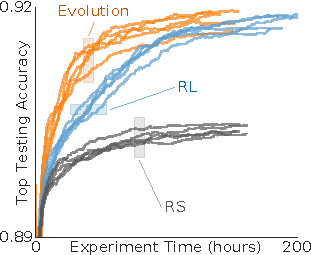
\includegraphics[scale=0.8]{AutoKeras_1}
	\end{subfigure}
	\begin{subfigure}{0.3\textwidth}
		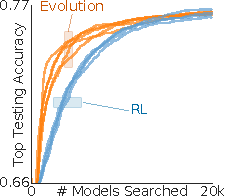
\includegraphics{AutoKeras_2}
	\end{subfigure}
	\begin{subfigure}{0.3\textwidth}
		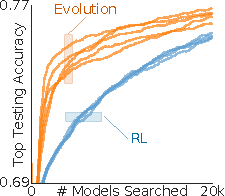
\includegraphics{AutoKeras_3}
	\end{subfigure}
	\caption{Reproduced figures from \citep{Jin2018} demonstrating effective reporting of NAS efficiency}
	\label{fig:reproduce}
\end{figure}
